\section{Theory}

\subsection{Overview of the Numerical Method}

We consider the reaction-diffusion equation
\[
  u_t \;=\; \mu\,u_{xx} \;+\; f(u),
  \quad x \in (0,L),\quad t>0,
\]
where \(\mu > 0\) is the diffusion coefficient and \(f(u)\) is a reaction term. We discretize
space by dividing \((0,L)\) into \(M+1\) subintervals of uniform width \(h = L/(M+1)\), so
the grid points are \(x_m = m\,h\) for \(m = 0,\dots,M+1\). In time, we use a step \(k>0\),
so \(t_n = n\,k\). Let \(U_m^n \approx u(x_m,t_n)\). Then we define the dimensionless
parameter
\[
  r \;=\; \frac{\mu\,k}{h^2}.
\]
The scheme combines a Crank–Nicolson-like step for the diffusion term with an explicit
component for the reaction. it approximates the spatial derivative at the midpoint between time steps.
It is unconditionally stable and second-order accurate in time and space. Concretely, each time-step consists of:

\begin{enumerate}
  \item \emph{Predictor}: approximate the diffusion term in a semi-implicit manner and
        add an explicit reaction increment:
        \[
          U_m^\star
          \;=\; U_m^n
          \;+\; \frac{r}{2}\bigl(\delta_x^2 U_m^\star + \delta_x^2 U_m^n\bigr)
          \;+\; k\,f\bigl(U_m^n\bigr), \quad \text{where} \quad \delta_x^2 U_m^n = U_{m+1}^n - 2\,U_m^n + U_{m-1}^n.
        \]


  \item \emph{Corrector}: apply a midpoint update for the reaction:
        \[
          U_m^{n+1}
          \;=\; U_m^\star
          \;+\; \tfrac{k}{2}\,\Bigl(f\bigl(U_m^\star\bigr) - f\bigl(U_m^n\bigr)\Bigr).
        \]
\end{enumerate}

Visually the scheme can be illustrated with a stencil as shown below. Clearly showing the discretization of
the domain and how this is used to calculate the next value in time with the diffusion term calculated
semi-implicitly and the reaction term explicity.


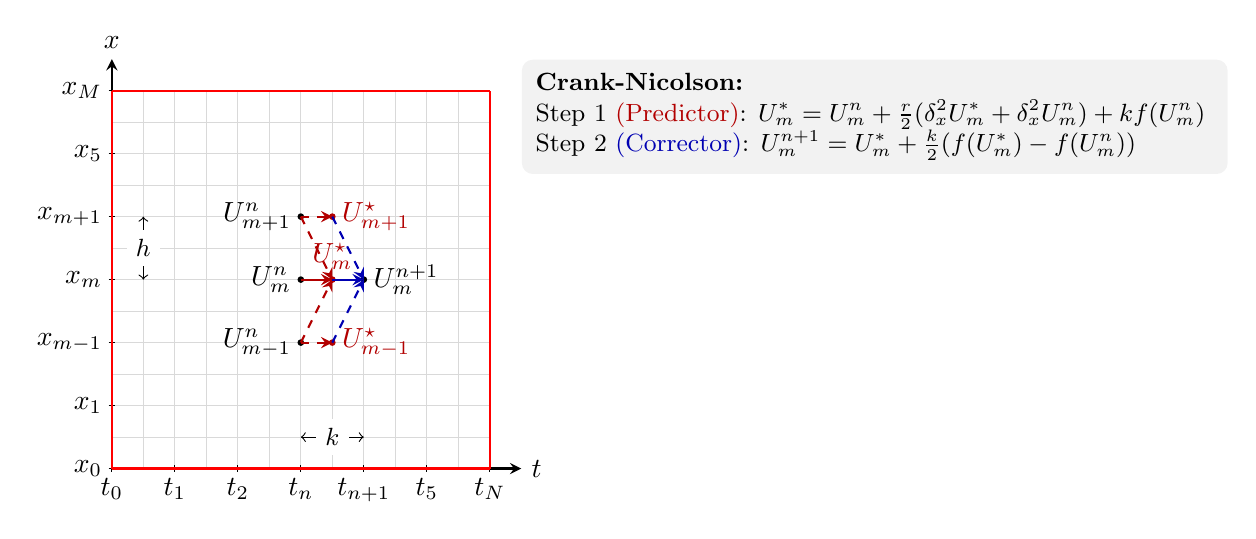
\begin{tikzpicture}[scale=0.8]
  % Define colors
  \colorlet{pointcolor}{black}
  \colorlet{gridcolor}{gray!30}
  \colorlet{predictorcolor}{red!70!black}
  \colorlet{correctorcolor}{blue!70!black}

  % Axes
  \draw[-stealth, thick] (0,0) -- (6.5,0) node[right] {$t$};
  \draw[-stealth, thick] (0,0) -- (0,6.5) node[above] {$x$};

  % Grid
  \draw[step=0.5cm, gridcolor, thin] (0,0) grid (6,6);

  % Add time labels
  \foreach \x/\label in {0/0, 1/1, 2/2, 3/n, 4/{n+1}, 5/5, 6/N} {
  \node[below] at (\x,0) {$t_{\label}$};
  \draw (\x,-0.05) -- (\x,0.05);
  }

  % Add space labels
  \foreach \y/\label in {0/0, 1/1, 2/{m-1}, 3/m, 4/{m+1}, 5/5, 6/M} {
  \node[left] at (0,\y) {$x_{\label}$};
  \draw (-0.05,\y) -- (0.05,\y);
  }

  % Highlight grid points for Crank-Nicolson stencil
  \fill[pointcolor] (3,3) circle (1.5pt) node[left] {$U_m^n$};
  \fill[pointcolor] (4,3) circle (1.5pt) node[right] {$U_m^{n+1}$};
  \fill[pointcolor] (3,2) circle (1.5pt) node[left] {$U_{m-1}^n$};
  \fill[pointcolor] (3,4) circle (1.5pt) node[left] {$U_{m+1}^n$};

  % Add intermediate points for the predictor step
  \fill[predictorcolor] (3.5,3) circle (1.5pt) node[above] {$U_m^\star$};
  \fill[predictorcolor] (3.5,2) circle (1.5pt) node[right] {$U_{m-1}^\star$};
  \fill[predictorcolor] (3.5,4) circle (1.5pt) node[right] {$U_{m+1}^\star$};

  % Show the predictor step with arrows
  \draw[->,-stealth, predictorcolor, thick] (3,3) -- (3.5,3);
  \draw[->,-stealth, predictorcolor, thick, dashed] (3,2) -- (3.5,3);
  \draw[->,-stealth, predictorcolor, thick, dashed] (3,4) -- (3.5,3);
  \draw[->,-stealth, predictorcolor, thick, dashed] (3,2) -- (3.5,2);
  \draw[->,-stealth, predictorcolor, thick, dashed] (3,4) -- (3.5,4);

  % Show the corrector step with arrows
  \draw[->,-stealth, correctorcolor, thick] (3.5,3) -- (4,3);
  \draw[->,-stealth, correctorcolor, thick, dashed] (3.5,2) -- (4,3);
  \draw[->,-stealth, correctorcolor, thick, dashed] (3.5,4) -- (4,3);

  % Step size annotations
  \draw[<->] (3,0.5) -- (4,0.5) node[midway, fill=white, font=\small] {$k$};
  \draw[<->] (0.5,3) -- (0.5,4) node[midway, fill=white, font=\small] {$h$};

  % Boundary and initial conditions
  \draw[red, thick] (0,0) -- (0,6);
  \draw[red, thick] (6,0) -- (6,6);
  \draw[red, thick] (0,0) -- (6,0);
  \draw[red, thick] (0,6) -- (6,6);

  % boundary labels MÅ FIKSES!

  % Crank-Nicolson scheme visualization
  \node[below right, align=left, font=\small, fill=gray!10, rounded corners, inner sep=5pt]
  at (6.5,6.5) {
  \textbf{Crank-Nicolson:}\\
  Step 1 \textcolor{predictorcolor}{(Predictor)}: $U_m^* = U_m^n + \frac{r}{2}(\delta_x^2 U_m^* + \delta_x^2 U_m^n) + k f(U_m^n)$ \hspace{5pt} \\
  Step 2 \textcolor{correctorcolor}{(Corrector)}: $U_m^{n+1} = U_m^* + \frac{k}{2}(f(U_m^*) - f(U_m^n))$
  };
\end{tikzpicture}

For the boundary conditions, either Dirichlet, Neumann, or Robin, one sets or solves for the boundary
values \(U_0^n\), \(U_{M+1}^n\) at each step as usual.

\subsection{Error Analysis}
To analyze the correctness of the scheme it is critical to determine both the consistency and stability of the
scheme. This is because a numerical method converges, as in, produces the true PDE solution as the grid is refined,
if and only if it is both consistent and stable. Consistency ensures the scheme’s discrete equations capture
the differential equation correctly. Stability ensures errors do not grow uncontrollably. Without both, one cannot
guarantee convergence.


\subsubsection{Consistency}
To determine the consistency of the modified Crank-Nicolson scheme for the PDE with the linear reaction term
$f(u) = au$, we analyze the local truncation error (LTE) by substituting the exact solution into our
numerical scheme.

\begin{theorem}{Local truncation error for the modified Crank-Nicolson}{lte_cn}
  For the PDE $u_t = \mu u_{xx} + au$ with constant $a$, the modified Crank-Nicolson scheme with steps $h$ (space)
  and $k$ (time) has local truncation error
  \[
    \|\tau_m^n\| = \mathcal{O}\!\left(k +\tfrac{h^4}{k}\right)
  \]
  where $u_m^n = u(x_m,t_n)$ is the exact solution and $U_m^n$ its numerical approximation.

  Under parabolic scaling $k \sim h^2$, the scheme achieves second-order accuracy:
  \[
    \|\tau_m^n\| = \mathcal{O}\!\left(h^2 + k^2\right)
  \]
\end{theorem}


\begin{proof}[Proof of Theorem~\ref{thm:lte_cn}]
  We analyze the truncation error by examining how the exact solution satisfies the numerical scheme.

  First, consider the central difference approximations for the second derivatives:
  \begin{align*}
    \delta_x^2 u_m^n     & = h^2u_{xx}(x_m,t_n) + \mathcal{O}(h^4)       \\
    \delta_x^2 u_m^\star & = h^2u_{xx}(x_m,t_n) + \mathcal{O}(h^4 + k^4)
  \end{align*}

  \textit{Step 1 (Predictor):} Substituting the exact solution into the first stage:
  \begin{equation}
    u_m^\star = u_m^n + \frac{r}{2}\left(\delta_x^2 u_m^\star + \delta_x^2 u_m^n\right) + kau_m^n = u_m^n + \frac{\mu k}{2}u_{xx}(x_m,t_n) + kau_m^n + \mathcal{O}(h^4 + k^4)
  \end{equation}
  \textit{Step 2 (Corrector):} For the second stage:
  \begin{align*}
    u_m^{n+1} & = u_m^\star + \frac{k}{2}(au_m^\star - au_m^n)
  \end{align*}

  From the PDE, we know $u_t = \mu u_{xx} + au$ and can derive expressions for higher time derivatives. Using Taylor expansion:
  \begin{align*}
    u(x_m,t_n+k) & = u_m^n + ku_t + \frac{k^2}{2}u_{tt} + \frac{k^3}{6}u_{ttt} + \mathcal{O}(k^4)
  \end{align*}

  Comparing this with our numerical solution, we obtain:
  \begin{align*}
    U_m^{n+1} - u_m^{n+1} & = \mathcal{O}(k^2 + h^4)
  \end{align*}

  The local truncation error per step is thus:
  \begin{align*}
    \|\tau_m^{n+1}\| & = \frac{|U_m^{n+1} - u_m^{n+1}|}{k} = \mathcal{O}\left(k + \frac{h^4}{k}\right)
  \end{align*}

  Under the parabolic scaling $k \sim h^2$, we have $\frac{h^4}{k} \sim h^2$, yielding second-order accuracy:
  \begin{align*}
    \|\tau_m^{n+1}\| = \mathcal{O}(h^2 + k^2)
  \end{align*}
\end{proof}

Hence, as stated in the theorem, if we choose \(k\) and \(h\) so that \(k \approx \mathrm{const}\times h^2\),
the method achieves second-order accuracy in both time and space.

\subsubsection{Stability Analysis}

We investigate whether the scheme can tolerate large time steps without amplification of numerical errors, thus
satisfing the conditions for stability.
For linear problems
\(\,u_t = \mu\,u_{xx} + a\,u,\) a von~Neumann analysis is done to see whether
this is true.

\begin{theorem}{von Neumann Stability for modified Crank--Nicolson}{von_neumann_cn}
  The modified Crank--Nicolson scheme for the PDE with a linear reaction term $f(u) = au$ is unconditionally
  stable for any choice of step sizes $h$ and $k$, as the amplification factor $\xi$ satisfies:
  \[
    |\xi| \leq 1 + Ck
  \]
  for some constant $C$ independent of step sizes.
\end{theorem}

\begin{proof}[Proof of Theorem~\ref{thm:von_neumann_cn}]
  We apply von Neumann stability analysis by studying how individual Fourier modes $U_m^n = \xi^n e^{i\beta mh}$
  evolve under our scheme, where $\beta$ is the wave number.

  As previously statet the PDE with a linear reaction term $f(u) = au$, the two-stage modified Crank--Nicolson
  scheme is given by:
  \begin{align*}
    U_m^\star & = U_m^n + \frac{r}{2}\left(U_{m+1}^\star - 2U_m^\star + U_{m-1}^\star + U_{m+1}^n - 2U_m^n + U_{m-1}^n\right) + kaU_m^n \\
    U_m^{n+1} & = U_m^\star + \frac{ka}{2}(U_m^\star - U_m^n)
  \end{align*}

  Substituting the Fourier mode $U_m^n = \xi^n e^{i\beta mh}$ and letting
  $U_m^\star = \xi^n \xi^\star e^{i\beta mh}$, we can use the identity
  $e^{i\beta (m+1)h} - 2e^{i\beta mh} + e^{i\beta (m-1)h} = -4\sin^2(\beta h/2)e^{i\beta mh}$ and derive:

  \begin{align*}
    \xi^\star & = \frac{1 - r\sin^2(\beta h/2) + ka}{1 + 2r\sin^2(\beta h/2)}
  \end{align*}

  For the second stage:
  \begin{align*}
    \xi^{n+1} & = \xi^n\left[\xi_\star\left(1 + \frac{ka}{2}\right) - \frac{ka}{2}\right]
  \end{align*}

  Therefore, the amplification factor is:
  \begin{align*}
    \xi & = \frac{\left(1 - r\sin^2(\beta h/2) + ka\right)\left(1 + \frac{ka}{2}\right) - \frac{ka}{2}\left(1 + 2r\sin^2(\beta h/2)\right)}{1 + 2r\sin^2(\beta h/2)}
  \end{align*}

  After algebraic simplification, and substituting $s = \sin^2(\beta h/2)$:
  \begin{align*}
    \xi & = \frac{1 - rs(1 + \tfrac{3}{2}ka) + ka + \tfrac{1}{2}k^2a^2}{1 + 2rs}
  \end{align*}

  Then for $a \geq 0$ and any $r > 0$, both numerator and denominator are positive with $\xi(s) < 1$ for all
  $s \in [0,1]$.

  \medskip

  For $a < 0$, the worst case occurs at $s = 0$, giving:
  \begin{align*}
    \xi(0) & = 1 + ka + \frac{k^2a^2}{2} = 1 + ka\left(1 + \frac{ka}{2}\right)
  \end{align*}

  For sufficiently small $k$:
  \begin{align*}
    |\xi(0)| & \leq 1 + |a|k(1 + |a|k/2)
  \end{align*}

  Therefore, $|\xi| \leq 1 + Ck$ with $C = |a|(1 + |a|k/2) \approx |a|$ for small $k$, confirming the scheme is unconditionally stable.
\end{proof}


\subsubsection{Global Error and Convergence}

\begin{theorem}{Lax Equivalence and Convergence of Crank--Nicolson}{cn_convergence}
  Since the modified Crank--Nicolson scheme is both consistent and stable, by the Lax Equivalence Theorem
  (Theorem~\ref{thm:lax}), it is convergent. Under the parabolic scaling $k \sim h^2$, the scheme achieves
  second-order convergence. Thus the global error satisfies:
  \[
    \|e_m^n\| = \mathcal{O}\!\left(h^2 + k^2\right)
  \]

\end{theorem}

Hence the proposed two-stage method inherits the main advantages of Crank--Nicolson (robust stability, second-order behavior) while treating the reaction term explicitly.

\subsection{Numerical Verification}
We verify the theoretical results by simulating the reaction-diffusion equation with a linear reaction term.
Here the reaction term is given by \(f(u) = au\) with \(a = 1\), and the diffusion coefficient is set to \(\mu = 1\).

\begin{figure}[H]
  \centering
  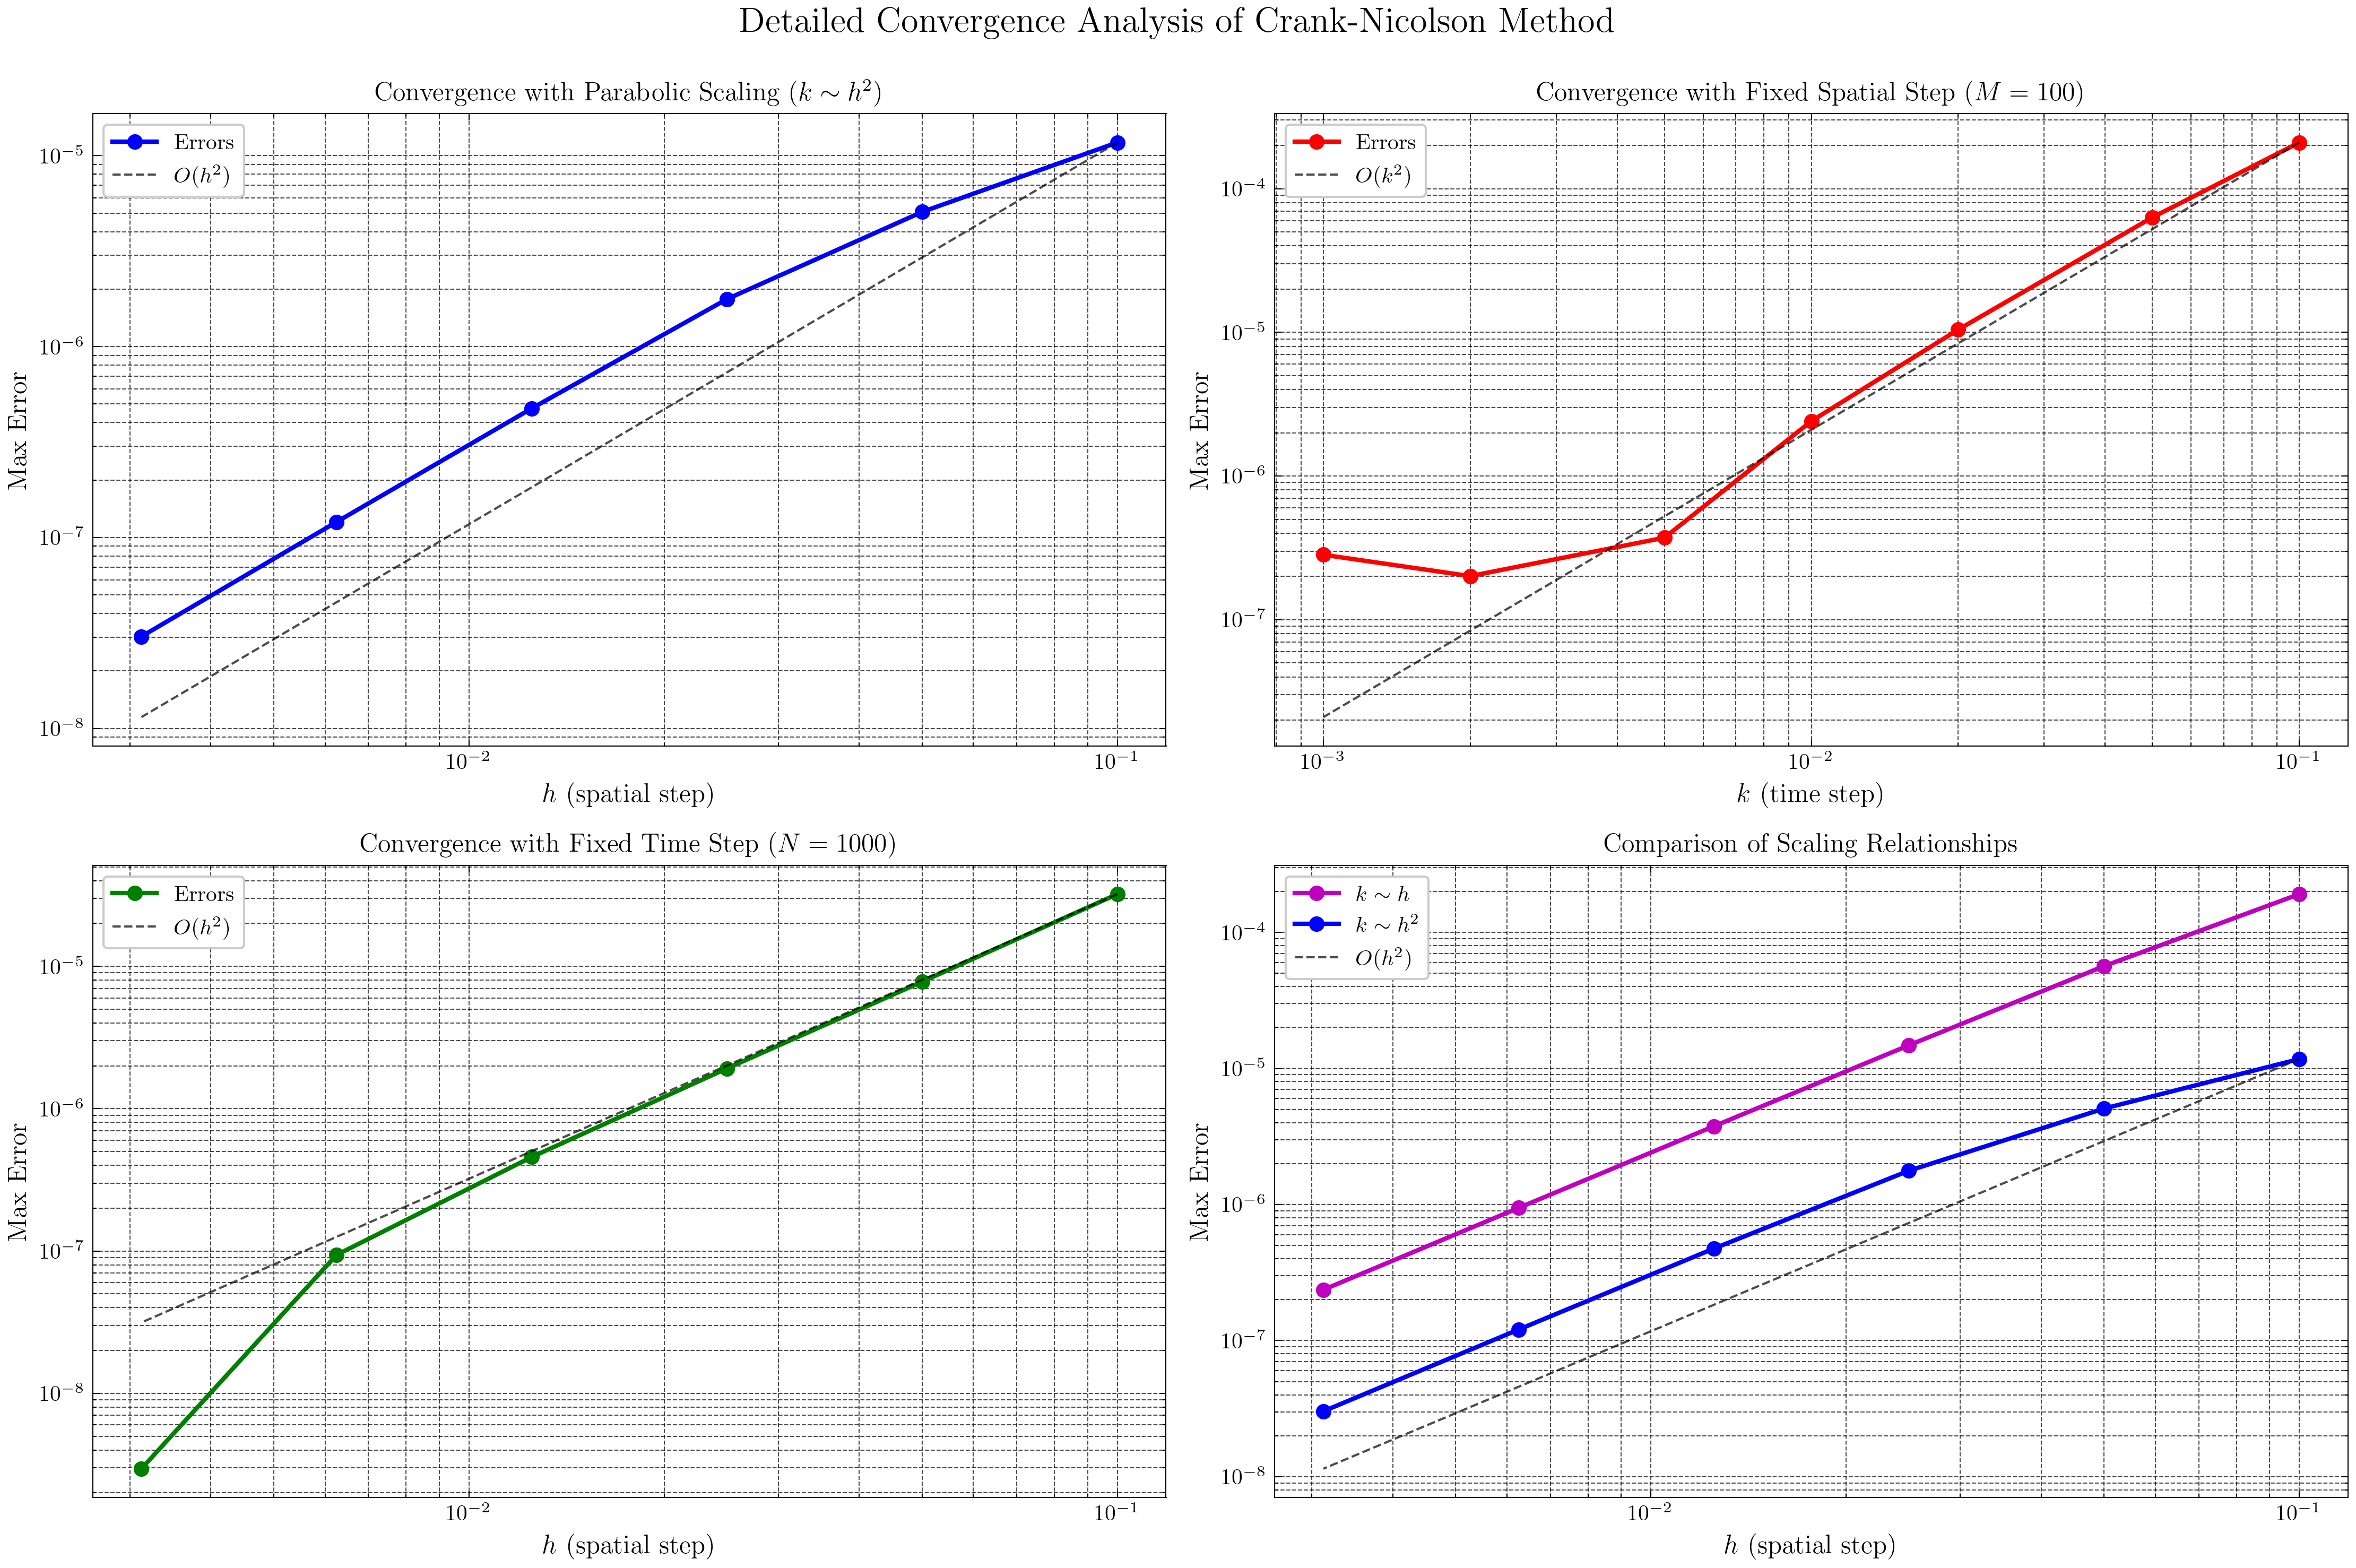
\includegraphics[width=0.5\textwidth]{figures/convergence_analysis_2d.png}
  \caption{Convergence analysis of the modified Crank--Nicolson scheme for the reaction-diffusion equation with a linear reaction term.}
  \label{fig:convergence_analysis_2d}
\end{figure}

The figure shows the convergence of the numerical solution to the exact solution as the grid is refined. The error decreases quadratically with respect to both \(h\) and \(k\), confirming the second-order accuracy of the scheme.

We can also confirm that choosing a parabolic scaling \(k \propto h^2\) yields second-order convergence.


